\documentclass{article}[12pt]
\usepackage[a4paper, margin=1in]{geometry}

% packages
%   formatting
%\usepackage[utf8]{inputenc}
\usepackage{url}
\usepackage{hyperref}
\hypersetup{
    colorlinks=true,
    linkcolor=blue,
    filecolor=magenta,      
    urlcolor=blue}
\usepackage{xcolor}
%\usepackage[T1]{fontenc}
%\usepackage{lmodern}
\usepackage{float}
%   math
\usepackage{amsmath}
\usepackage{amssymb}
%\usepackage{bbm}

%\usepackage{mathptmx}
%\usepackage{verbatim}
%\usepackage{bm}
%   figures, tables, ...
\usepackage{algpseudocode}
\usepackage{algorithm}
\usepackage{graphicx}
\usepackage{booktabs}
%\usepackage{multirow}%http://ctan.org/pkg/multirow

% python
\usepackage{listings}
\definecolor{darkgreen}{rgb}{0,0.6,0}
\lstdefinestyle{Python}{
    showstringspaces=false,
    language        = Python,
    basicstyle      = \small\ttfamily,
    morekeywords = {as},
    keywordstyle    = \color{blue},
    stringstyle     = \color{darkgreen},
    commentstyle    = \color{darkgreen}\ttfamily,
	breaklines = true,
	postbreak=\text{$\hookrightarrow$\space},
	% style >>> and ... 
	%   see: https://tex.stackexchange.com/questions/326655/make-a-keyword-in-listings-enviorment
	alsoletter = {>,.} ,
    morekeywords = [2]{>>>,...},
    keywordstyle = [2]\color{cyan}\bfseries}

% bibliograpy
\usepackage{biblatex}
\addbibresource{ags.bib}
\addbibresource{main.bib}

% macros
\input ags.tex
\newcommand{\bvarepsabs}{\boldsymbol{\varepsilon}_\text{abs}}
\newcommand{\bvarepsrel}{\boldsymbol{\varepsilon}_\text{rel}}
\newcommand{\varepsabs}{\varepsilon_\text{abs}}
\newcommand{\varepsrel}{\varepsilon_\text{rel}}

\newcommand{\AGSComment}[1]{{\color{cyan} Aleksei: #1}}
\newcommand{\JRComment}[1]{{\color{violet} Jag: #1}}
\newcommand{\FJH}[1]{{\color{purple}#1}}
\newcommand{\scnote}[1]{ {\textcolor{blue}  {\mbox{SC: } #1}}}

% metadata
\title{Quasi-Monte Carlo for Vector Functions of Integrals}
\author{Aleksei Sorokin, Jagadeeswaran Rathinavel}
\date{\today}


\begin{document}

\maketitle

\begin{abstract}
Quasi-Monte Carlo methods present an efficient approach for multivariate numerical integration. Algorithms exist to adaptively sample the integrand until a user defined error tolerance is satisfied with theoretical guarantees or with high probability. This work describes our extension of such methods to support adaptive sampling to satisfy error criteria for vector functions of multiple integrals. Although several functions involving multiple integrals are being evaluated, only one low discrepancy sequence is required, albeit sometimes of larger dimension than the integration domain. These enhanced algorithms are implemented in the QMCPy Python package with support for vectorized, economical integrand evaluation. We exemplify these capabilities with examples from machine learning including the approximation of acquisition function values for Bayesian Optimization, coefficients for Bayesian logistic regression, and sensitivity indices for both hyperparameters and input features.
\end{abstract}

\tableofcontents

\newpage 

\AGSNote{

\section*{Notes}

TODO 
\begin{itemize}
    \item replace violation function $V$ with infinite bounds
    \item flip boolean flags so True means sufficient approximation and False requires further computation
    \item new PyPI release
\end{itemize}
MISC
\begin{itemize}
    \item Efficient estimation of the ANOVA mean dimension, with an application to neural net classification. Christopher R. Hoyt Stanford University. Art B. Owen Stanford University December 2020
\end{itemize}
}

\newpage

\section{Introduction}

Many quantities of interest may be formulated as functions of multiple integrands. For example, we may be interested in computing the expected value of a random function at multiple locations. In other examples we may be interested in computing the ratio of two integrals.

Monte Carlo (MC) methods have proven to be an efficient technique for high dimensional numerical integration. Quasi-Monte Carlo (QMC) offers even greater efficiency over crude Monte Carlo for integrands with low effective dimension \AGSNote{cite}. Numerous MC and QMC methods have been developed to adaptively sample an integrand and construct error bounds that hold absolutely or with high probability for nicely behaved integrands. 

This work extends some existing QMC methods to adaptively approximate a function of multiple integrands to within a user-specified error tolerance. Our extension leverages shared samples, custom error bound propagation, multi-dimensional vectorization, and parallel function evaluation. The resulting routines are implemented into the QMCPy Python package \cite{QMCPy} which is distributed on both GitHub and PyPI. 

\section{Monte Carlo Methods}

Monte Carlo methods are well-suited to approximate the expected value a random variable. Suppose we would like to approximate the vector mean $\bmu = \bbE[f(X)] \in \bbR^\rho$ where $X\sim\calU(0,1)^d$ and  $f: [0,1]^d \to \bbR^\rho$ is a vectorized objective function such that $f(\cdot)=(f_1(\cdot),\dots,f_\rho(\cdot))$.  Crude Monte Carlo computes the approximation 
\begin{equation}
    \label{eq:mcapprox}
    \hat{\bmu} = \frac{1}{n}\sum_{i=1}^n f(\bx_i) \approx \int_{[0,1]^d}f(\bx)\D\bx = \bmu
\end{equation}
using $\bx_1,\dots,\bx_n \in [0,1]^d$. While the standard uniform choice for $X$ may seem restrictive, a variety of distributions are compatible in this framework after an appropriate variable transformation, see \cite{QMCSoftware} for details.

Crude Monte Carlo methods choose sampling nodes to be independent and identically distributed (IID). That is, $\bx_1,\dots,\bx_n \simiid \calU[0,1]^d$.
The error in approximating $\bmu$ by $\hat{\bmu}$ based on IID nodes is  $\calO(n^{-1/2})$. 

Quasi-Monte Carlo (QMC) methods choose sampling nodes in a carefully coordinated manner to avoid the gaps and clusters observed in IID nodes.  Discrepancy measures quantify how closely the discrete distribution of such points matches a target distribution. QMC nodes have low discrepancy (LD) with the standard uniform distribution compared to IID nodes. Popular LD node sets include the Halton points, digital nets, and integration lattices \AGSNote{cite}. The error in approximating $\bmu$ by $\hat{\bmu}$ based on LD nodes is  $\calO(n^{-1+\delta})$ where $0 < \delta \ll 1/2$. This convergence rate for QMC methods is significantly faster than the rate for crude Monte Carlo when $f(X)$ has low effective dimension, see \AGSNote{cite}. 

The QMC methods in this article rely on LD sequences that are extensible in both dimension and number of samples. This enables our algorithms to utilize shared point sets and adaptively increase the number of points used to estimate $\hat{\bmu}$ without needing to discard previous observations. For more on extensible LD sequence see \AGSNote{cite}. Such LD sequences are often implemented in base 2 for computational efficiently and therefore prefer sampling at the first $2^m$ nodes in the sequence to attain low discrepancy measures. Thus, existing QMC algorithms tend to iteratively  double the sample size until the error bounds on $\bmu$ are sufficiently tight. 

The remainder of this article focuses on extending the functionality of existing QMC methods. Crude Monte Carlo methods may be extended in a similar way to accommodate integrands with higher effective dimension. We defer this task to future development.  For a more carefully treatment of crude Monte Carlo and Quasi-Monte Carlo see \cite{mcbook}. 

\section{Monte Carlo Approximation Error}\label{sec:Existing_QMC_Methods}

In this section we assume $f$ is a scalar function and discuss existing Monte Carlo methods for approximating error bounds on a single mean $\mu$. Specifically, given $n$ samples $\bx_1,\dots,\bx_n$ and  corresponding function evaluations $f(\bx_1),\dots,f(\bx_n)$ we discuss methods for estimating lower bound $\mu^-$ and upper bound $\mu^+$ so that $\mu \in [\mu^-,\mu^+]$ either guaranteed or with high probability. 

The following error estimation techniques are implemented, among others, into the open source QMC library QMCPy. Table \ref{table:qmcpy_sc} tabulates algorithm features discussed next.

\begin{table}[H]
\begin{tabular}{r c c c}
    QMCPy Class & Guaranteed Error Estimation & Compatible Points\\
    \hline
    \texttt{CubMCCLT} \AGSNote{cite} & & \texttt{IID} \\
    \texttt{CubMCG} \cite{cubmcg} & X & \texttt{IID} \\
    \texttt{CubQMCCLT} \AGSNote{cite} & & \texttt{LD} \\
    \texttt{CubQMC\{Net,Lattice\}G} \cite{cubqmcsobol,cubqmclattice} & X & \texttt{DigitalNetB2}, \texttt{Lattice} \\
    \texttt{CubQMCBayes\{Net,Lattice\}G} \AGSNote{cite} \cite{cubqmcbayeslattice} & X &  \texttt{DigitalNetB2}, \texttt{Lattice} \\
    \hline
\end{tabular}
\caption{A comparison of select Monte Carlo and Quasi-Monte Carlo stopping criterion algorithms available in QMCPy.}
\label{table:qmcpy_sc}
\end{table}

\texttt{CubMCCLT: } When $\bx_1,\dots,\bx_n$ are IID and $f$ has finite variance, the Central Limit Theorem provides a $100(1-\alpha)\%$ confidence interval for $\mu$ by setting $\mu^\pm = \hat{\mu} \pm Z^{1-\alpha/2}\sigma/\sqrt{n}$. Here $\sigma$ is the standard deviation of $f(X)$, which is generally unknown, $Z^{1-\alpha/2}$ is the inverse CDF of the standard normal distribution at $1-\alpha/2$, and $\hat{\mu}$ is the sample average of function evaluations as in \eqref{eq:mcapprox}. Often $\sigma$ is approximated by the unbiased estimator $S = \sqrt{1/(n-1)\sum_{i=1}^n(f(\bx_i)-\hat{\mu})^2}$, perhaps multiplied by an inflation factor $C>1$ for a more conservative approximation. The tractable error bounds on $\mu$ are then
\begin{equation}
    \mu^\pm = \hat{\mu} \pm \frac{CZ^{1-\alpha/2}S}{\sqrt{n}}
    \label{eq:clt_mu_bounds}.
\end{equation}

\texttt{CubMCG: } The Central Limit Theorem produces probabilistic bounds on $\mu$ which relies on the sample size approaching infinity and the unverifiable assumption that $\sigma \leq CS$. If $f(X)$ has a known upper bound on the kurtosis $\kappa = \bbE[(f(X)-\mu)^4]/\sigma^4-3$, then   \cite{cubmcg} provides a guaranteed fixed width confidence interval $[\mu^-,\mu^+]$ for $\mu$ based on IID nodes and the Berry-Esseen Inequality.

\texttt{CubQMCCLT: } Finding QMC bounds for $\mu$ tends to be more difficult due to the deterministic nature of LD sequences. One idea is to produce $R$ IID randomizations of a LD sequence which preserve low discrepancy and then use bounds based on the $R$ IID sample averages. Specifically, let $\bx_{1,r},\dots,\bx_{n,r}$ be an IID randomization of a deterministic LD point set and let $\hat{\mu}_r = 1/n \sum_{i=1}^n f(\bx_{i,r})$ for $r=1,\dots,R$. Then using the pooled mean estimate $\hat{\mu} = 1/R \sum_{r=1}^R \hat{\mu}_r$ we may approximate $100(1-\alpha/2)\%$ confidence bounds on $\mu$ to be
\begin{equation}
    \mu^\pm = \hat{\mu} \pm t_{R-1}^{1-\alpha/2}S_r
    \label{eq:qmc_clt_mu_bounds}
\end{equation}
where $S_r = \sqrt{R^{-1}(1-R)^{-1}\sum_{i=1}^R(\hat{\mu}_r - \hat{\mu})^2}$ and $t_{R-1}^{1-\alpha/2}$ is the inverse CDF of the student T distribution with $R-1$ degrees of freedom. More information on this method can be found in \cite[Chapter 17]{mcbook} or \cite{qmc4pde_preprint}.

\texttt{CubQMC\{Net,Lattice\}G: }While \eqref{eq:qmc_clt_mu_bounds} provides intuitive, practical bounds, this approximation requires $Rn$ function evaluations which may be prohibitively large.  \citeauthor{cubqmclattice} overcome this challenges by developing algorithms that track the decay of Fourier coefficients based on a single randomized LD sequence ($R=1$) \cite{adaptive_qmc}. These algorithms provide guaranteed error bounds on $\bmu$ for functions lying within an appropriately parameterized cone by tracking the decay of either the Walsh coefficients for digital sequences \cite{cubqmcsobol} or the complex exponential Fourier coefficients for integration lattices \cite{cubqmclattice}.  

%%
%% TODO: Compare cubQMCBayes against cubQMC algorithms
%% For What kind of integrands, Bayes algos work better

\texttt{CubQMCBayes\{Net,Lattice\}G: } Another pair of QMC algorithms take a Bayesian approach to error estimation. Rather than assume the function lies within a cone, these algorithms assume the integrand is an instance of a Gaussian process. Utilizing special kernels matched to LD sequences allows fast approximation of Gaussian process hyperparameters and provides guaranteed error estimation. These Bayesian QMC algorithms are also available for both digital nets \AGSNote{cite} and integration lattices  \cite{cubqmcbayeslattice}.

\section{Optimal Approximation of a Combined Solution}

Given an appropriate set of  samples and their corresponding function evaluations, the QMC stopping criterion discussed in the previous section are easily vectorized to produce bounds on the individual means $\bmu \in \bbR^\rho$ such that $\bmu \in [\bmu^-,\bmu^+]$ either guaranteed or with high probability. We are interested in approximating a combined solution $s \in \bbR$ which is a function of individual means $\bmu$.  The next section generalizes the solution $s$ from a scalar to a to multi-dimensional array with special attention to enable economical computation.

In order to approximate $s$, the user is required to define functions $C^-,C^+: \bbR^\rho \times \bbR^\rho \to \bbR$ which combine individual bounds $\bmu^-,\bmu^+$ into a combined bounds $s^-,s^+$ respectively so that $s \in [s^-,s^+]$ with the same guarantee or high likelihood. For example, if we are interested in approximating the product of two expectations $s=\mu_1\mu_2$, then we may set
\begin{align*}
    s^- &= C^-(\bmu^-,\bmu^+) = \min_{\mu \in [\bmu^-,\bmu^+]} \mu_1\mu_2 = \min(\mu_1^-\mu_2^-,\mu_1^-\mu_2^+,\mu_1^+\mu_2^-,\mu_1^+\mu_2^+), \\
    s^+ &= C^+(\bmu^-,\bmu^+) = \max_{\mu \in [\bmu^-,\bmu^+]} \mu_1\mu_2 = \max(\mu_1^-\mu_2^-,\mu_1^-\mu_2^+,\mu_1^+\mu_2^-,\mu_1^+\mu_2^+).
\end{align*}
If $s^-=-\infty$ or $s^+=\infty$, then we automatically determine the error criterion has not been met and proceed with subsequent sampling. This situation arises, for example, when computing the ratio of integrals and the bounds on the denominator include 0. Going forward, we assume $s^-,s^+$ are finite. 

We now wish to derive an optimal solution approximation $\hat{s}$ with respect to some error threshold $\varepsilon$ and  error metric $h(s,\varepsilon)$. Here we assume $h(\cdot,\varepsilon)$ is a metric map, so for any $s,\tilde{s} \in \bbR$ we have $\lvert h(s,\varepsilon) - h(\tilde{s},\varepsilon) \rvert \leq \lvert s - \tilde{s} \rvert$. Error metric options include
\begin{subequations}
\begin{align}
    h(s,\varepsilon) & = \varepsilon \quad &&\text{absolute error satisfied}, \label{eq:h_abs}\\
    h(s,\varepsilon) &= \max\left(\varepsabs,\lvert s \rvert \varepsrel \right) \quad &&\text{absolute or relative error satisfied, and } \label{eq:h_abs_or_rel} \\
    h(s,\varepsilon) &= \min\left(\varepsabs,\lvert s \rvert \varepsrel \right) \quad &&\text{absolute and relative error satisfied.} \label{eq:h_abs_and_rel}
\end{align}
\end{subequations}
%Note that the optimal approximation $\hat{s}$ is not necessarily the midpoint of the combined solution bounds $s^-,s^+$.
Define $g(s,\hat{s},\varepsilon)=\lvert s - \hat{s} \rvert -h(s,\varepsilon)$ and note that the error criterion is met if and only if 
\begin{equation*}
    \max_{s \in [s^-,s^+]} g(s,\hat{s},\varepsilon) \leq 0.
\end{equation*}
So for all $s \in [s^-,s^+]$ we have either
\begin{align*}
    g(s^-,\hat{s},\varepsilon)-g(s,\hat{s},\varepsilon) 
    &= \lvert s^- - \hat{s} \rvert -h(s^-,\varepsilon) - \lvert s - \hat{s} \rvert  + h(s,\varepsilon) \\
    &\geq s - s^- - \lvert h(s,\varepsilon)-h(s^-,\varepsilon) \rvert  %\JRComment{\text{is it supposed to be} \lvert s - s^- \rvert} % because $s >= s^-$
    \\
    &\geq 0 \qquad \text{if } s^- \leq s \leq \hat{s}, \text{ or} \\
    g(s^+,\hat{s},\varepsilon)-g(s,\hat{s},\varepsilon) 
    &= \lvert s^+ - \hat{s} \rvert -h(s^+,\varepsilon) - \lvert s - \hat{s} \rvert  + h(s,\varepsilon) \\
    &\geq s^+ - s - \lvert h(s,\varepsilon)-h(s^+,\varepsilon) \rvert \\
    &\geq 0 \qquad \text{if } \hat{s} \leq s \leq s^+.
\end{align*}
This means that $g(\cdot,\hat{s},\varepsilon)$ attains its maximum at either $s^-$ or $s^+$ so that
\begin{equation*}
    \max_{s \in [s^-,s^+]} g(s,\hat{s},\varepsilon) = \max g(s^\pm,\hat{s},\varepsilon) = \max\left(g(s^-,\hat{s},\varepsilon) \;,\; g(s^+,\hat{s},\varepsilon)\right).
\end{equation*}
The function $g(s^-,\cdot,\varepsilon)$ is monotonically decreasing for $\hat{s} < s^-$ and monotonically increasing for $\hat{s} > s^-$. Similarly, $g(s^+,\cdot,\varepsilon)$ is monotonically decreasing for $\hat{s} < s^+$ and monotonically increasing for $\hat{s} > s^+$. This means that the optimal choice of $\hat{s}$ to minimize $\max g(s^\pm,\hat{s},\varepsilon)$ lies in $[s^-,s^+]$ and satisfies
\begin{align}
    g(s^-,\hat{s},\varepsilon) &= g(s^+,\hat{s},\varepsilon) \nonumber \\
    \therefore \quad \hat{s} - s^- - h(s^-,\varepsilon) &= s^+ - \hat{s} - h(s^+,\varepsilon) \nonumber \\ 
    \therefore \quad \hat{s} &= \frac{1}{2}\left[ s^- + s^+ +h(s^-,\varepsilon) - h(s^+,\varepsilon) \right]. \label{eq:shat_opt}
\end{align}

Under this optimal choice of $\hat{s}$, 
\begin{equation*}
    \label{eq:g_under_shat_opt}
    2 \max g(s^\pm,\hat{s},\varepsilon) =  s^+  -  s^-  - h(s^-,\varepsilon) - h(s^+,\varepsilon).
\end{equation*}
Therefore, our error criterion is satisfied if and only if
\begin{equation}
    s^+-s^-<h(s^-,\varepsilon)+h(s^+,\varepsilon).
    \label{eq:sc}
\end{equation}
% If $s^- < 0 < s^+$, then \eqref{eq:h_abs_and_rel} cannot hold since $h(s,\varepsilon) \le \lvert s \rvert \varepsrel$, and so
% \begin{equation}
% 2 \max g(s^\pm,\hat{s},\varepsilon) \ge s^+ (1 - \varepsrel) - s^- (1  - \varepsrel) = (s^+ - s^-)(1 - \varepsrel) > 0.
% \end{equation}
% If $s^- < 0 < s^+$ and $\varepsabs = 0$ for \eqref{eq:h_abs_or_rel}, then $h(s,\varepsilon) = \lvert s \rvert \varepsrel$, and again \eqref{eq:h_abs_and_rel} cannot be satisfied.

\section{Vectorized QMC Algorithm} \label{sec: Vectorized Implementation}

In the previous section we assumed that individual solutions $\bmu \in \bbR^\rho$ were used to compute a single combined solution $s \in \bbR$. We now relax these assumptions to enable approximation of multi-dimensional combined solutions $\bs \in \bbR^{\bseta}$ from multi-dimensional individual solutions $\bmu \in \bbR^{\brho}$ via error thresholds $\bvarepsilon \in \bbR_+^{\bseta}$. Here the bold superscript is a vector of dimensions so that, for example, if $\bs$ is a $2 \times 3$ matrix then $\bseta = (2,3)$. The optimal approximation $\hat{\bs}$ may still be computed by \eqref{eq:shat_opt} where functions are assumed to be appropriately vectorized. Similarly, \eqref{eq:sc} may be used to compute Boolean flags $\bb \in \tfset^\eta$ where $b_{\bi}=\True$ if and only if the error criterion is satisfied for the combined solution at multi-index $\bi$. 

To be evaluation efficient, the user may define a dependency function $D: \tfset^{\bseta} \to \tfset^{\brho}$ which maps error criterion flags on the combined solutions to flags on individual solutions. In the next batch of samples, we pass $f$ the individual flags $\tilde{\bb} = D(\bb)$ so the integrand may avoid evaluating outputs at indices contributing to an already sufficiently approximated combined solution. In a simple example, if $\bmu=\bs$ then $D$ may be defined as the identity map. Then, when $\bs_{\bi}=\True$ at some iteration, $f$ need not evaluate index ${\bi}$ outputs in future evaluations. 

Algorithm \ref{algo:qmcsc} details the typical QMC stopping criterion included in QMCPy. The cost of this algorithm is concentrated in evaluating $f$ at $2^m$ points with a cost we assume to be $\$(f)2^m$. In practice, this cost may be smaller if $f$ can take advantage of not having to produce all outputs for every iteration. The compute time may also be reduced through parallel evaluation of a function $f$ which is slow to evaluate. It should be noted that for functions which are quick to evaluate, the overhead of multi-processing parallelization may increase compute time.

\begin{algorithm}[h!]
    \caption{\ct{QMC Stopping Criterion} \\ Operations are understood to act elementwise.}
    \label{algo:qmcsc}
    \begin{algorithmic}
    \Require $f: [0,1]^{n \times d} \times \tfset^{\brho} \to \bbR^{n \times \brho}$, an integrand capable of being evaluated at sampling locations $X \in [0,1]^{n \times d}$ with individual flags $\tilde{\bb} \in \tfset^{\brho}$ to compute $n$ evaluations without computing outputs where $\tilde{b}_{\bi}=\True$.
    \Require $m_0$, where $2^{m_0}$ is the initial number of samples.
    \Require $\text{GenLD}: \bbN \times \bbN \to [0,1]^{n \times d}$, an appropriate generator of randomized LD samples taking in starting index $n_\text{start}$ and final index $n_\text{end}$ (not inclusive) and returns the $n = n_\text{end} - n_\text{start}$ samples in those positions of the sequence. 
    \Require $C^-,C^+: \bbR^{\brho} \times \bbR^{\brho} \to \bbR^{\bseta}$, functions transforming bounds on the individual solutions into bounds on the combined solution
    \Require $\bvarepsilon \in \bbR_+^{\bseta}$, a non-negative error tolerance. 
    \Require $D: \tfset^{\bseta} \to \tfset^{\brho}$, a dependency function mapping stopping criterion flags for the combined solutions to flags for individual solutions. 
    \Require $h: \bbR^{\bseta} \times \bbR^{\bseta}_+ \to \bbR^{\bseta}$, an error metric function, see for example \eqref{eq:h_abs}, \eqref{eq:h_abs_or_rel}, or \eqref{eq:h_abs_and_rel}
    \Require $\text{UpdateIndividualBounds}: [0,1]^{n \times d} \times \bbR^{n \times \brho} \to \bbR^{\brho} \times \bbR^{\brho}$, a function computing $\bmu^-,\bmu^+$ from sampling locations $X \in [0,1]^{n \times d}$, function evaluations $\by \in \bbR^{n \times \brho}$, and data stored from previous calls. See Section \ref{sec:Existing_QMC_Methods} for examples. 
    
    \hrulefill
    
    \State $n_\text{start} \gets 0$
    \State $n_\text{end} \gets 2^{m_0}$
    \State $\tilde{\bb} \gets \False^{\brho}$
    \State $\bb \gets \False^{\bseta}$
    \While{$\exists \bi$ where $\tilde{b}_i = \False$}
        \State $X \gets \text{GenLD}(n_\text{start},n_\text{end})$
        \State $\by \gets f(X,\tilde{\bb})$
        \State $\bmu^+,\bmu^- \gets \text{UpdateIndividualBounds}(X,\by)$
        \State $\bs^- = C^-(\bmu^-,\bmu^+)$
        \State $\bs^+ = C^+(\bmu^-,\bmu^+)$
        \State $\hat{\bs} \gets \frac{1}{2}\left[\bs^-+\bs^++h(\bs^-,\bvarepsilon)-h(\bs^+,\bvarepsilon)\right]$
        \State $\bb \gets \text{Boolean}(\bs^+-\bs^- < h(\bs^-,\bvarepsilon)+h(\bs^+,\bvarepsilon))$
        \State $\tilde{\bb} \gets D(\bb)$
        \State $n_\text{start} \gets n_\text{end}$
        \State $n_\text{end} \gets 2n_\text{start}$
    \EndWhile
    \end{algorithmic}
\end{algorithm}

\section{Examples}

\subsection{Vectorized Acquisition Functions for Bayesian Optimization}

\subsection{Bayesian Logistic Regression}

Consider a model with predictor $\bx = (1,x_1, \dots, x_{d-1}) \in \bbR^d$ and binary response $y \in \{0,1\}$. Logistic regression models the probability of observing $y = 1$ given $\bx$ to $P(y=1;\bx) = \left(1+\exp(-\bs.\bx)\right)^{-1}$ where $\bs \in \bbR^d$ is the coefficient vector of model parameters which we are interested in approximating.

A normal prior on $\bs$ with prior mean $\bnu$ and prior covariance $\mSigma$ yields the prior density
$$P(\bs) = \frac{\exp\left(-(\bs-\bnu)^T\mSigma^{-1}(\bs-\bmu)/2\right)}{\sqrt{(2\pi)^d\lvert \mSigma\rvert}}.$$ Now, suppose we have observed $N$ responses $y_1,\dots,y_N$ at IID sampling locations $\bx_1,\dots,\bx_N$. Then the likelihood of these observations given coefficients $\bs$ is
\begin{equation*}
    P(y_1,\dots,y_N ; \bs) = \prod_{i=1}^N \left(\frac{\exp(\bs.\bx_i)}{1+\exp(\bs.\bx_i)}\right)^{-y_i} \left(1-\frac{\exp(\bs.\bx_i)}{1+\exp(\bs.\bx_i)}\right)^{1-y_i} = \prod_{i=1}^N \frac{\exp(\bs.\bx_i)^{y_i}}{1+\exp(\bs.\bx_i)}
\end{equation*}
By Bayes' Theorem, the posterior density of $\bs$ is 
$$P(\bs;y_1,\dots,y_N) = \frac{P(y_1,\dots,y_N;\bs)P(\bs)}{P(y_1,\dots,y_N)} = \frac{P(y_1,\dots,y_N;\bs)P(\bs)}{\int_{\bbR^d} P(y_1,\dots,y_N;\bs)P(\bs)\D\bs}.$$
We approximate $\bs$ to be the posterior mean
\begin{equation}
    \bbE[\bs;y_1,\dots,y_N] = \frac{\int_{\bbR^d}\bs P(y_1,\dots,y_N;\bs)P(\bs)\D\bs}{\int_{\bbR^d}P(y_1,\dots,y_N;\bs)P(\bs)\D\bs}. \label{eq:bayes_posterior_mean}
\end{equation}

Set $\bmu \in \bbR^{2 \times d}$ so that $\mu_{1j} = \int_{\bbR^d}s_j P(y_1,\dots,y_N;\bs)P(\bs)\D\bs$ and $\mu_{2j} = \int_{\bbR^d}P(y_1,\dots,y_N;\bs)P(\bs)\D\bs$ for $j=1,\dots,d$. Here $\mu_{21},\dots,\mu_{2d}$ all copy the marginal likelihood in order to store different estimates of $P(y_1,\dots,y_N)$ for different $s_j$ for economical computation.  Then, for $j=1,\dots,d$,  the quantity of interest from \eqref{eq:bayes_posterior_mean} becomes $\bbE[s_j;y_1,\dots,y_N] = \mu_{1j}/\mu_{2j}$ and we set

\begin{align*}
    s_j^- = C_j^-(\bmu^-,\bmu^+) &= \min_{\bmu \in [\bmu^-,\bmu^+]} \frac{\mu_{1j}}{\mu_{2j}} = 
    \begin{cases}
        -\infty, & 0 \in [\mu_{2j}^-,\mu_{2j}^+] \\
        \min\left(\frac{\mu_{1j}^-}{\mu_{2j}^-},\frac{\mu_{1j}^+}{\mu_{2j}^-},\frac{\mu_{1j}^-}{\mu_{2j}^+},\frac{\mu_{1j}^+}{\mu_{2j}^+}\right), & \text{else}
    \end{cases}, \\
    s_j^+ = C_j^+(\bmu^-,\bmu^+) &= \max_{\bmu \in [\bmu^-,\bmu^+]} \frac{\mu_{1j}}{\mu_{2j}} =
    \begin{cases}
        \infty, & 0 \in [\mu_{2j}^-,\mu_{2j}^+] \\
         \max\left(\frac{\mu_{1j}^-}{\mu_{2j}^-},\frac{\mu_{1j}^+}{\mu_{2j}^-},\frac{\mu_{1j}^-}{\mu_{2j}^+},\frac{\mu_{1j}^+}{\mu_{2j}^+}\right), & \text{else}
    \end{cases}.
\end{align*}
Moreover, we set the dependency function $D: \tfset^d \to \tfset^{2 \times d}$ to stack two copies of combined flag rows so that 
\begin{equation*}
    D(\bb) =  \begin{pmatrix} \bb \\ \bb \end{pmatrix}.
\end{equation*}

\subsubsection{Haberman's Dataset Example}

Here we perform logistic regression on the Haberman's Survival Dataset retreived from the UCI Machine Learning Repository \cite{uci_ml_repo}. This dataset concerns a study between 1958 and 1970 at the University of Chicago's Billings Hospital that tracked the survival of patients five years after undergoing treatment for breast cancer. Predictors include the age of patient at the time of operation, operation year after 1900 e.g. 65 is 1965, and number of positive axillary nodes detected. The binary response variable indicates the patients survival status five years after the operation. 

We use 2/3 of the dataset for training and the remaining 1/3 for testing. The training set has 151 positive records and 54 negative records while the testing set has 74 positive records and 27 negative records. The class imbalance reflects the fact that most patients in the study survived longer than 5 years after the operation. Since we value identifying at risk patients, we seek models with a low number of false negative predictions i.e. we desire models with high recall. Table \ref{tab:lr_models} compares a Bayesian logistic model against logistic regression models fit with an Elastic net regularization penalty
$$\min_{\bs,c} \left[\frac{1-\lambda}{2} \lVert \bs \rVert_2^2 + \lambda \lVert \bs \rVert_1+C\sum_{i=1}^N\log(\exp(-y_i(\bx_i.\bs+c))+1)\right]$$
where $C>0$ constant and $\lambda \in [0,1]$ controls the trade-off between $l_1$ and $l_2$ regularization. The Elastic-Net models were fit using the scikit-learn Python package with the ``saga'' optimizer \cite{scikit-learn}. The Bayesian logistic regression model was fit with $\bvarepsabs=.05$, $\bvarepsrel=.5$, error metric $h$ matching \eqref{eq:h_abs_and_rel}. Note that the Bayesian logistic regression model has the highest test recall metric.  

\begin{table}[H]
    \centering
    \begin{tabular}{l|rrrr|rrr}
        Method &\multicolumn{4}{|c|}{Coefficients} &\multicolumn{3}{c}{Test Metrics \%}\\
        {} &       Age &  1900 Year &  Axillary Nodes &  Intercept &  Accuracy &  Precision &   Recall \\
        \midrule
        % begin insert
        Elastic-Net $\lambda=0.0$ & -1.23e-02 &   3.44e-02 &       -1.15e-01 &   1.99e-03 &     74.3 &      76.7 &   93.2 \\
        Elastic-Net $\lambda=0.5$ & -1.20e-02 &   3.42e-02 &       -1.15e-01 &   2.03e-03 &     74.3 &      76.7 &   93.2 \\
        Elastic-Net $\lambda=1.0$ & -1.18e-02 &   3.39e-02 &       -1.14e-01 &   2.06e-03 &     74.3 &      76.7 &   93.2 \\
        Bayesian                & -4.14e-03 &   1.30e-01 &       -1.57e-01 &   8.03e-03 &     74.3 &      74.0 &  100.0 \\
        % end insert
        \bottomrule
    \end{tabular}
    \caption{Comparison of Logistic regression models for the Haberman dataset.}
    \label{tab:lr_models}
\end{table}
\subsection{Sensitivity Indices}

Sensitivity analysis quantifies how uncertainty in a functions output may be attributed to subsets of function inputs. Functional ANOVA (analysis of variance) decomposes an objective function $f \in L^2((0,1)^d)$ into the sum of orthogonal functions $(f_u)_{u \subseteq 1:d}$. Here $1:d$ denotes the set of all dimensions $\{1,\dots,d\}$ and $f_u \in L^2((0,1)^{\lvert u \rvert})$ denotes a sub-function dependent only on inputs $\bx_u = (x_j)_{j \in u}$. By construction, these sub-functions sum to the objective function so that
\begin{equation}
    f(\bx) = \sum_{u \subseteq 1:d} f_u(\bx_u) \label{eq:fanova}
\end{equation}
\cite[Appendix A]{mcbook}. The orthogonality of sub-functions enables the variance of $f$ to be decomposed into the sum of variances of sub-functions. Specifically, denoting the variance of $f$ by $\sigma^2$, we may write
\begin{equation*}
    \sigma^2 = \sum_{u \subseteq 1:d} \sigma^2_u
\end{equation*}
where $\sigma^2_u$ is the variance of sub-function $f_u$. The sub-variance $\sigma_u$ directly quantifies the variance of $f$ attributable to inputs $u \subseteq 1:d$.  The \emph{closed and total Sobol' indices},
\begin{equation}
    \label{eq:sobol_indices}
    \underline{\tau}_u^2 = \sum_{v \subset u} \sigma^2_v \quad \text{and} \quad 
    \overline{\tau}_u^2 = \sum_{v \cap u \neq \emptyset} \sigma^2_v,
\end{equation}
quantify the variance attributable to subsets of $u$ and subsets containing $u$ respectively. The \emph{sensitivity indices},
\begin{equation}
    \label{eq:sensitivity_indices_og}
    \underline{s}_u = \underline{\tau}_u^2/\sigma^2 \quad \text{and} \quad 
    \overline{s}_u = \overline{\tau}_u^2/\sigma^2,
\end{equation}
normalize the Sobol' indices to quantify the proportion of variance explained by a given subset of inputs. 

Suppose one is interested in computing the closed and total sensitivity indices of $f$ at $u_1,\dots,u_k \in 1:d$.  Then we may choose the individual solutions $\bmu \in \bbR^{6 \times k}$ and combined solutions $\bs \in \bbR^{2 \times k}$ where, for $j=1,\dots,k$,
\begin{align*}
    \mu_{1j} &= \underline{\tau}_{u_j}^2 = \int_{[0,1]^{2d}} f(\bx)[f(\bx_{u_j},\bz_{-{u_j}})-f(\bz)]\D\bx\D\bz \\
    \mu_{2j} &= \overline{\tau}_{u_j}^2 = \frac{1}{2}\int_{[0,1]^{2d}} [f(\bz)-f(\bx_u,\bz_{-{u_j}})]^2\D\bx\D\bz \\
    \mu_{3j} &= \mu_{4j} = \int_{[0,1]^d} f(\bx)\D\bx, \\
    \mu_{5j} &= \mu_{6j} = \int_{[0,1]^d} f^2(\bx)\D\bx, \\
    s_{1j} &= \underline{s}_{u_j} = \frac{\underline{\tau}_{u_j}^2}{\sigma^2} = \frac{\mu_{1j}}{\mu_{5j}-\mu_{3j}^2}, \qquad \text{and} \\
    s_{2j} &= \overline{s}_{u_j} = \frac{\overline{\tau}_{u_j}^2}{\sigma^2} = \frac{\mu_{2j}}{\mu_{6j}-\mu_{4j}}.
\end{align*}
Here the notation
\begin{equation}
    (\bx_{u},\bz_{-u}) = \left(\begin{aligned}x_{j}, \quad & j \in u \\ z_{j}, \quad & j \notin u \end{aligned}\right)_{j=1}^d
\end{equation}
denotes a point with inputs $u$ from $\bx$ and inputs $-u=(1:d)\cap u^c$ from $\bz$.
For $\bmu$, the first row contains closed Sobol' indices, the second row contains total Sobol' indices, the third / forth row contain copied first moments of $f$, and the forth / fifth row contain copied second moments of $f$. As in the previous section, we have copied various individual solutions to maintain separate estimates of the first / second moments for each combined solution. For $\bs$, the first row contains closed sensitivity indices while the second row contains total sensitivity indices. 

Then bounds from individual to combined solutions may be transformed via $C^-,C^+:\bbR^{6 \times k} \to \bbR^{2 \times k}$ defined, for $j=1,\dots,k$, by  
\begin{align*}
    C_{1j}^-(\bmu^-,\bmu^+) 
    &= \text{clip}\left(\min_{\bmu \in [\bmu^-,\bmu^+]} \frac{\mu_{1j}}{\mu_{5j}-\mu_{3j}^2}\right) \\
    &= \begin{cases} 
        \text{clip}\left(\min\left(\frac{\mu_{1j}^-}{\mu_{5j}^+-\left(\mu_{3j}^-\right)^2},\frac{\mu_{1j}^-}{\mu_{5j}^+-\left(\mu_{3j}^+\right)^2}\right)\right), & \mu_{5j}^- - \left(\mu_{3j}^\pm\right)^2 >0 \\
        0, &\text{else}
    \end{cases} \\
    C_{1j}^+(\bmu^-,\bmu^+) 
    &= \text{clip}\left(\max_{\bmu \in [\bmu^-,\bmu^+]} \frac{\mu_{1j}}{\mu_{5j}-\mu_{3j}^2}\right) \\
    &= \begin{cases} 
        \text{clip}\left(\max\left(\frac{\mu_{1j}^+}{\mu_{5j}^--\left(\mu_{3j}^-\right)^2},\frac{\mu_{1j}^+}{\mu_{5j}^--\left(\mu_{3j}^+\right)^2}\right)\right), & \mu_{5j}^- - \left(\mu_{3j}^\pm\right)^2 >0 \\
        1, &\text{else}
    \end{cases}
\end{align*}
where $\text{clip}(\cdot) = \min(1,\max(0,\cdot))$ restricts values between 0 and 1. Similarly, we may compute $C_{2j}^-$ by replacing indices 1,3,5 in $C_{1j}^-$ with indices 2,4,6 respectively and likewise for computing $C_{2j}^+$ from $C_{1j}^+$. Above, we have simplified the bounds using the facts that sensitivity indices are between 0 and 1, the variance of $f$ is non-negative, and Sobol' indices are non-negative. 

Moreover, the dependency function $D:\tfset^{2 \times k} \to \tfset^{6 \times k}$ may be defined to vertically stack combined flags three times to produce individual flags so that 
\begin{equation*}
    D(\bb) = \begin{pmatrix} \bb \\ \bb \\ \bb \end{pmatrix}.
\end{equation*}
In the QMCPy implementation we further generalize to allow objective functions $f:[0,1]^d \to \bbR^{\tilde{\brho}}$ so that $\brho = (6,k,\tilde{\brho})$ and $\bseta = (2,k,\tilde{\brho})$.

Sensitivity indices present an important special case for computational complexity. Say our QMC algorithm takes $2^m$ total samples to accurately approximate closed and total sensitivity indices for $(u_j)_{j=1}^k \subseteq 1:d$. Then the computational cost is $\$(f)(2+k)2^m$ since every time our sensitivity index function is evaluated at $\tilde{\bx} = (\bx,\bz) \in [0,1]^{2d}$ we must evaluate the users objective function at $f(\bx)$, $f(\bz)$, and $f(\bx_{u_j},\bz_{-{u_j}})$ for $j=1,\dots,k$. Also note that when $f$ is defined to take samples in  $[0,1]^d$ to outcomes in $\bbR^{\tilde{\brho}}$, sensitivity index approximation requires a wrapper taking samples in $[0,1]^{2d}$ to outcomes in $\bbR^{\brho}$

If a user is only interested in approximating singleton sensitivity indices, $u_j = \{j\}$ for $j=1,\dots,d$, then it is possible to reduce the cost from $\$(f)(2+d)2^m$ to $\$(f)2^{m+1}$ using order $1$ replicated designs \cite{alex2008comparison,tissot2015randomized}. Such designs have been extended to  Sobol' sequences \AGSNote{(digital nets?)} in \cite{replicated_designs_sobol_seq} and utilized for sensitivity index approximation in \cite{reliable_sobol_indices_approx}. In the future, we plan to optimize QMCPy to utilize replicated designs when the opportunity arises.

\subsubsection{Ishigami Function Example}

The Ishigami function \cite{ishigami1990importance} is defined for $T \sim \calU(-\pi,\pi)^3$ as
\begin{equation*}
    g(T) = \left(1+bT_3^4\right)\sin(T_1) + a\sin^2(T_2).
\end{equation*}
After a change of variables we may equivalently define the Ishigami function as 
$f(X) = g\left(\pi(2X-1)\right)$ where $X \sim \calU(0,1)^3$. 

Figure \ref{fig:ishigami_fu} shows exact functional ANOVA sub-functions $f_u$ for select $u \in 1:d$ and Figure \ref{fig:ishigami} shows approximate sensitivity indices for the Ishigami function. 

\begin{figure}[H]
    \centering
    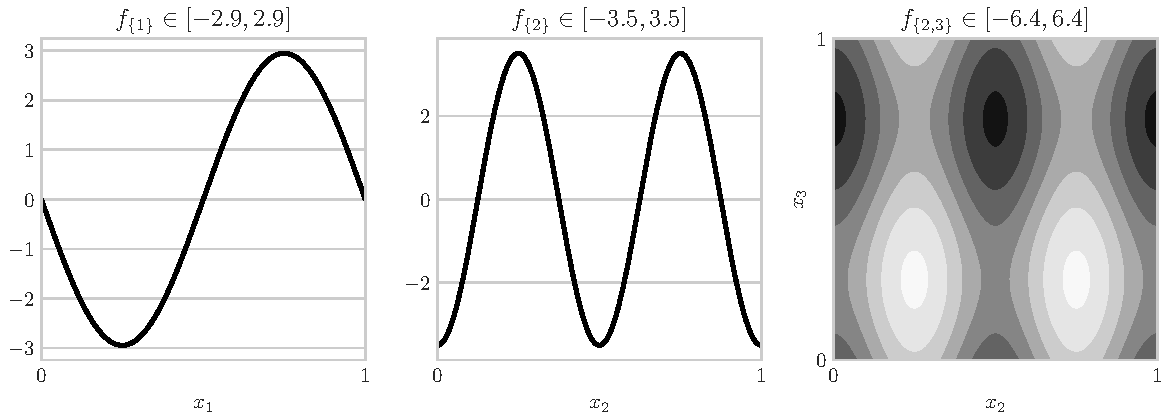
\includegraphics[width=.8\textwidth]{figs/ishigami_fu.pdf}
    \caption{True Ishigami sub-functions $f_u$ for $u \in 1:d$ from \eqref{eq:fanova}.}
    \label{fig:ishigami_fu}
\end{figure}

\begin{figure}[H]
    \centering
    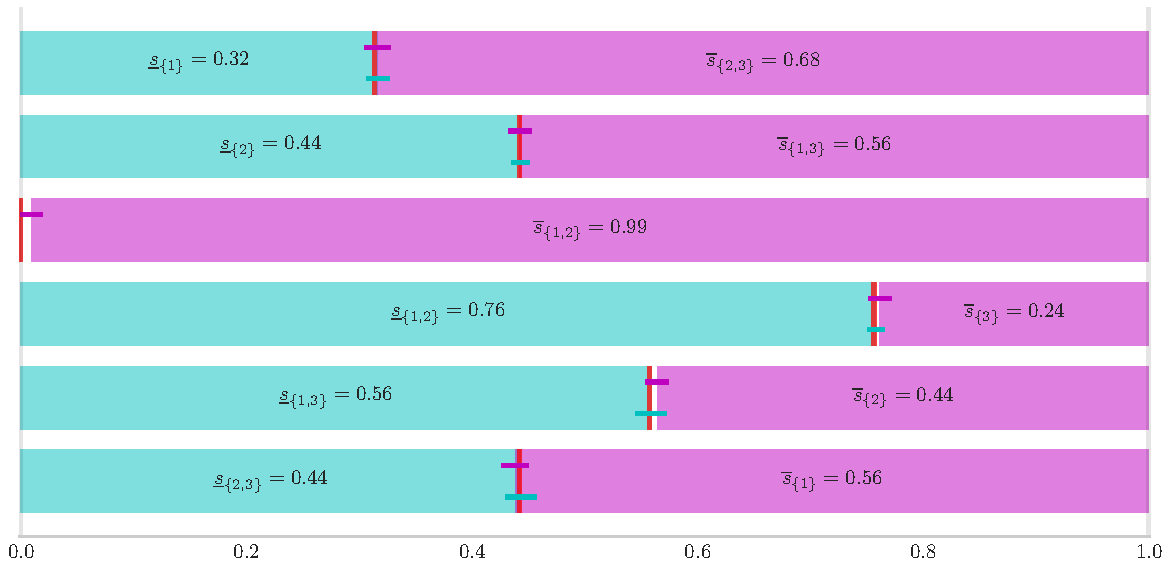
\includegraphics[width=.8\textwidth]{figs/ishigami.pdf}
    \caption{Approximate closed and total sensitivity indices for the Ishigami function illustrating the relationship $\underline{s}_u + \overline{s}_{u^c} = 1$ for $u \in 1:d$.}
    \label{fig:ishigami}
\end{figure}

\AGSNote{\subsubsection{Machine Learning Examples}}

%\AGSNote{Maybe use the decision trees for iris dataset from \url{https://github.com/QMCSoftware/QMCSoftware/blob/iris/demos/iris.ipynb}. The results aren't that impressive since Iris is a pretty small dataset and sensitivity indices are somewhat automatic for decision trees. I'd like to do something like we have in this notebook though. This paper could include one or both of the analysis procedures. Hyperparameter importance is interesting, but currently doesn't have a lot of actionable results. Feature importance is more interesting / relevant, I'm leaning towards this. Art Owen and Chris Hoyt have done something similar for neural networks which is pretty interesting. Including both would be ideal (but time consuming).}

\AGSNote{\section{Conclusions and Future Work}}

\printbibliography

\iffalse
\AGSNote{

$h(\bs,\bvarepsilon)$ Holder continuous such that $\Delta_\rho\left(h(\bs,\bvarepsilon),h(\tilde{\bs},\bvarepsilon)\right) \leq C \Delta_\gamma^\alpha\left(\bs,\tilde{\bs}\right)$ for all $\bs,\tilde{\bs} \in \bbR^\gamma$ where $\Delta_\rho$ and $\Delta_\gamma$ are two distance metrics on $\bbR^\rho$ and $\bbR^\gamma$ respectively. 

Define $g(\bs,\hat{\bs},\bvarepsilon) = \Delta_\gamma(\bs,\hat{\bs}) - h(\bs,\bvarepsilon)$ to be how fall short the approximation error falls from the error tolerance. When $$\max_{[\bs \in \bs^-,\bs^+]} g(\bs,\hat{\bs},\bvarepsilon) \leq 0$$
the error tolerance has been satisfied.

For all $\bs \in [\bs^-,\bs^+]$,

\begin{align*}
    
\end{align*}

}

\AGSNote{
NEI / QEI Demo from Mike McCourt on qmcpy.org

https://arxiv.org/pdf/1807.02811.pdf

http://proceedings.mlr.press/v70/wang17e/wang17e.pdf

https://proceedings.neurips.cc/paper/2020/file/6fec24eac8f18ed793f5eaad3dd7977c-Paper.pdf

https://www.jmlr.org/papers/volume20/18-225/18-225.pdf

http://proceedings.mlr.press/v139/malkomes21a.html


http://proceedings.mlr.press/v124/lee20a.html
}

\fi
\end{document}
